\section{Simulation Analysis and the Path for the Greater Good}

For this analysis, we used the default diode model available in \textit{Ngspice}, having then created the circuit presented in Fig. \ref{fig:bigscheme} (it was using Ngspice that we determined, in fact, what was the best circuit for our purposes). So, we used the following chain of thought in order to do what we did. In the envelope detector part, we took the limit as $R \rightarrow \infty$, which is the same as no current passing through there, which is the same as nothing being there. This drastically reduces our ripples, for then we do not need the resistance at all and the cost is 0. Of course this is slightly counterbalanced by the presence of the $10^{-6}$, in the merit calculation (\eqref{score}).  Knowing that the voltage ripples reduce to \eqref{eq:ripples}
\begin{equation}
    V_{ripple} = v_o(0) - v_o(T) = A \left(1 - e^{-\frac{T}{2RC}}\right)
    \label{eq:ripples}
\end{equation}
we can model very superficially the function that should describe this merit in terms of our components (\eqref{eq:approx}).

\begin{equation}
    f(R,C) = \frac{1}{(R+C)*A*\left(1 - e^{-\frac{T}{2RC}}+ 10^{-6}\right )}
    \label{eq:approx}
\end{equation}

From that, we can then plot what's the aspect of the function, shown in Fig. \ref{fig:plot2}.

\begin{figure}[H]
    \centering
    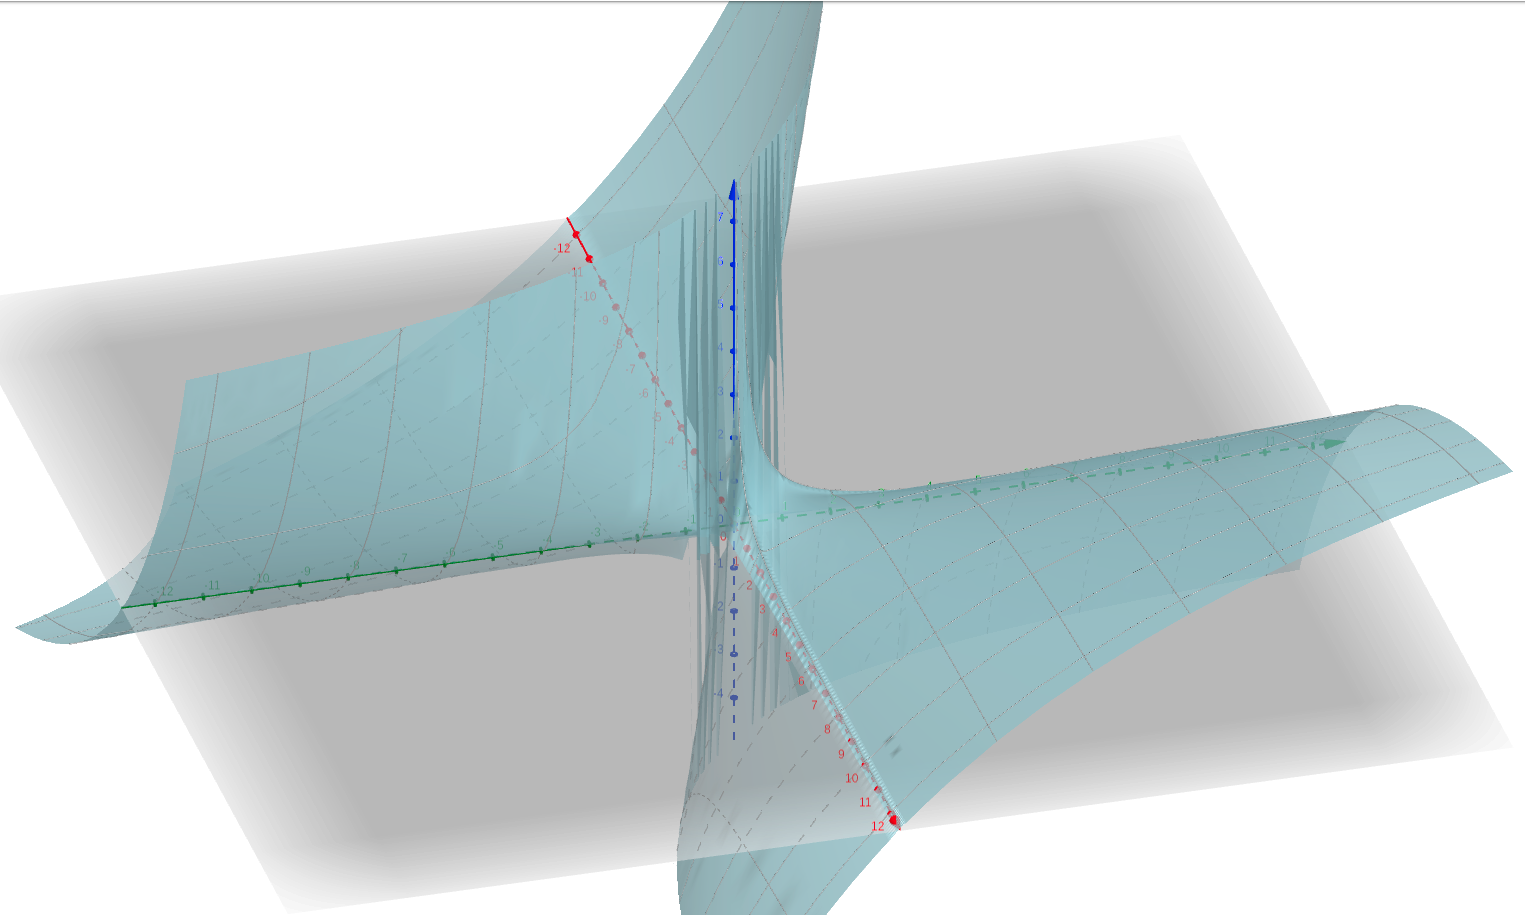
\includegraphics[width = 0.85\linewidth]{cost.png}
        \caption{\textit{Merit approximated function. Plot obtained using GeoGebra3D}}
    \label{fig:plot2}
\end{figure}

And thus we have the justification of our doings by removing the resistor. Then, we made use of the specifications of the non-linear part of the diodes and found that there is a very fortunate correlation between the amount of diodes in the voltage regulator and the ripples in the end voltage (we basically substitute our R by the incremental resistor arising from the diode series). What this means is that we can let go of the equation that says that $R2$ must be much greater than $rd$, for this is but a very rough approximation of the real life's diode behaviour. The only setback of this method is the stabilization time, but the merit does not take that into account, so we're good. This way, we used 31 diodes, for nonetheless we did not want to have an exaggerated stabilization time. WARNING: This will cause big differences between the theoretical analysis and the simulation. The model presented in class, when applied to Octave, will basically serve of nothing.

Finally, one found the values considered as the best to find an optimal merit score which are given by:

\begin{table}[H]
    \centering
    \begin{tabular}{|c|c|c|c|}
    \hline
        \textbf{Component} &  \textbf{Amount} & \textbf{Value} & \textbf{Cost}\\
        \hline
        \hline
        Resistors & 1 & $0.2k\Omega$ & 0.2\\
        \hline
        Capacitors & 1 &  $1.33\mu$F & 1.33\\
        \hline
        Diodes & 31+4 & - & 3.5 \\
        \hline
    \end{tabular}
    \caption{Components values shown in Fig. \ref{fig:bigscheme}.}
    \label{tab:tentativas}
\end{table}


\subsection{Cost and Merit Score}
Evaluating the merit, and knowing that the cost is given by \eqref{eq:cost}
\begin{equation}
    c = cost = 35 \cdot 0.1 + 0.2 + 1.33 =  5.03\text{MU}
    \label{eq:cost}
\end{equation}

Using the values obtained for $c$, $d$ and $r$, one can finally calculate the merit score obtained with this circuit (calculated using equation \eqref{score}), which allows one to get the following score:

\begin{table}[H]
    \centering
    \begin{tabular}{|c|c|}
          \hline
          @gb[i] & 8.369438e-18\\ \hline
@r1[i] & 7.979758e-18\\ \hline
@r2[i] & -8.36944e-18\\ \hline
@r3[i] & 3.896799e-19\\ \hline
@r4[i] & -1.73508e-18\\ \hline
@r5[i] & -2.79994e-03\\ \hline
@r6[i] & 1.301043e-18\\ \hline
@r7[i] & 8.876953e-19\\ \hline
v(1) & 0.000000e+00\\ \hline
v(2) & 8.298505e-15\\ \hline
v(3) & 2.570053e-14\\ \hline
v(5) & 7.105427e-15\\ \hline
v(6) & 8.403629e+00\\ \hline
v(7) & -2.64534e-15\\ \hline
v(8) & -3.55271e-15\\ \hline
cfp1 & -2.64534e-15\\ \hline

          \hline
    \end{tabular}
    \caption{Merit.}
    \label{tab:fresnel}
\end{table}

\subsection{Envelope Detector and Voltage Regulator output voltages}
To understand the role played by the envelope detector and the voltage regulator circuits in our circuit one plotted the results obtained for the output voltages in each one of them. So, starting by the plot obtained at the output terminals of the envelope detector circuit

\begin{equation}
    V = v_4
\end{equation}

Plotting this function:

\vspace{-140px}
\begin{figure}[H]
    \centering
    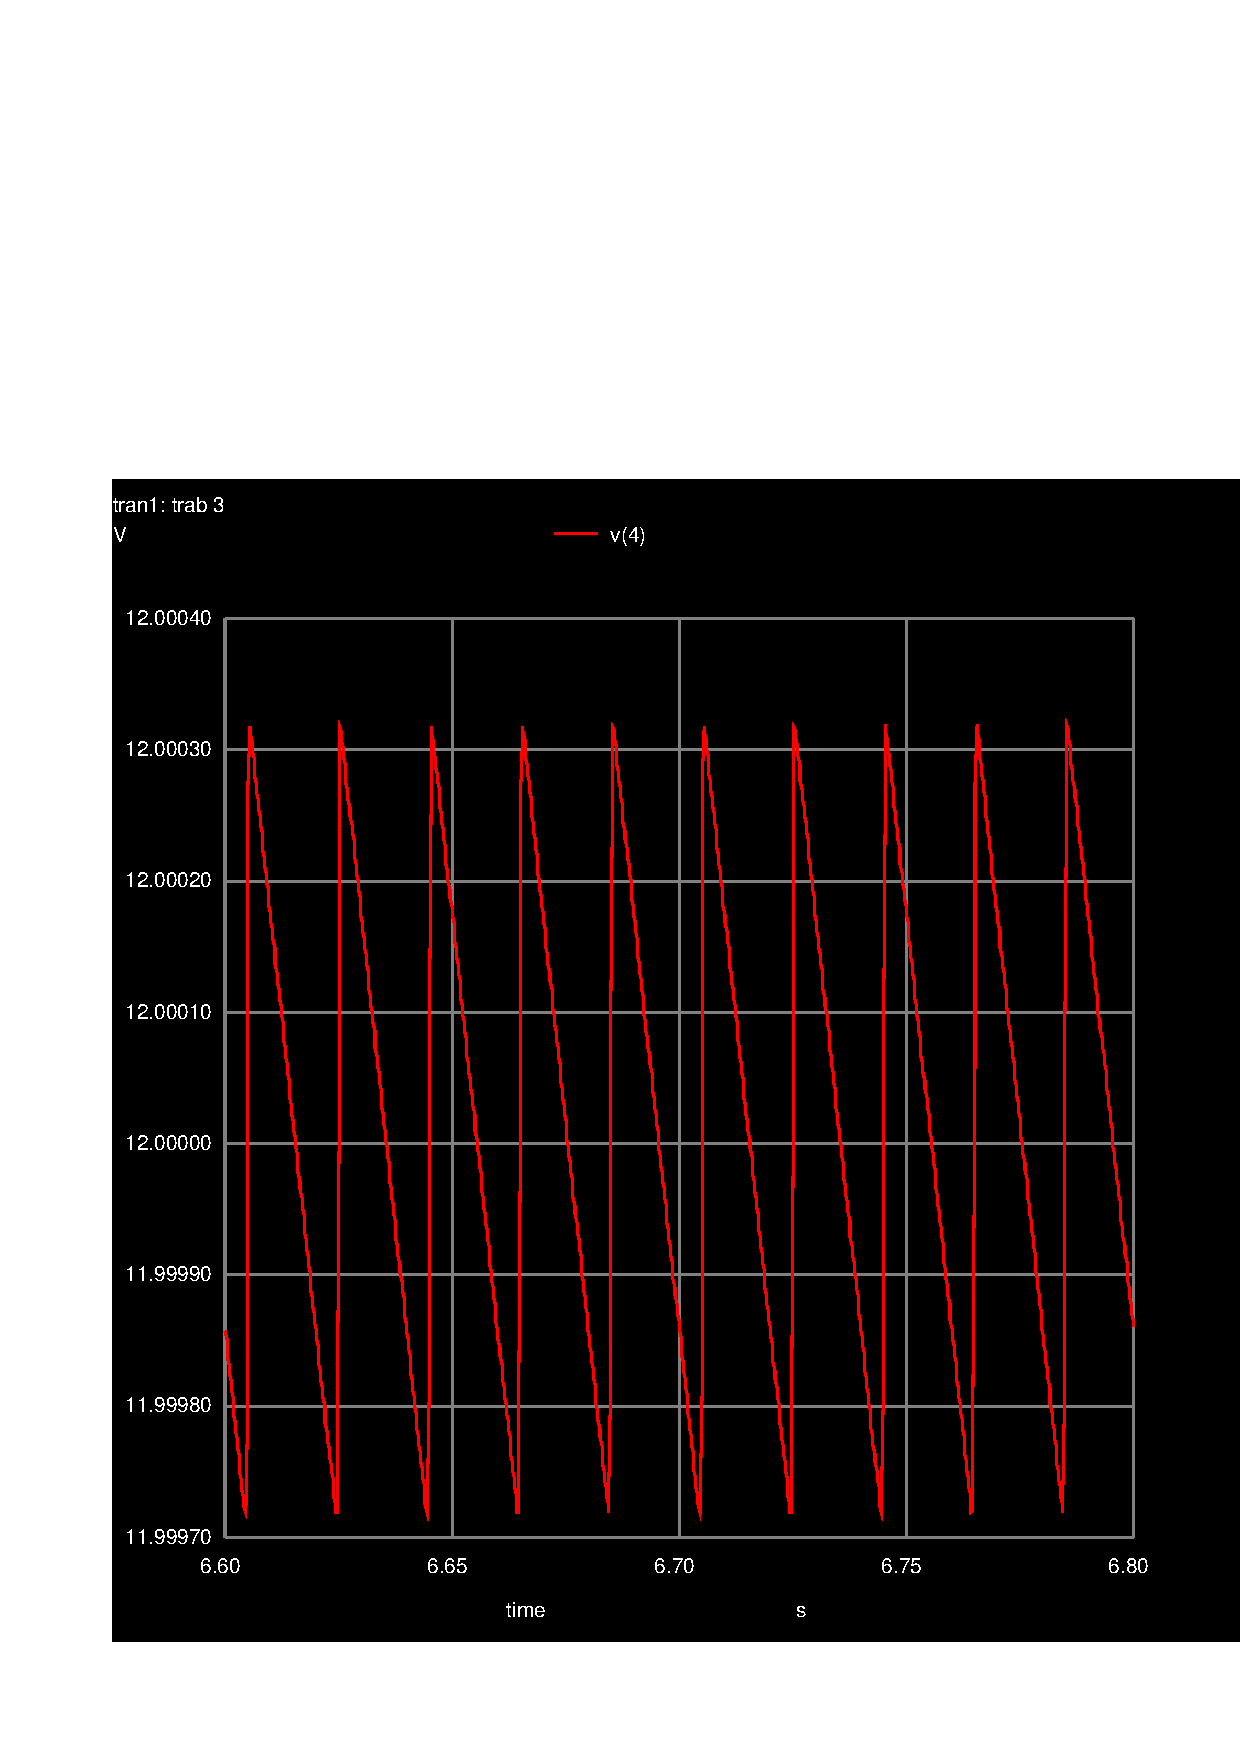
\includegraphics[width = 0.85\linewidth]{sim/antes.pdf}
    \vspace*{-10mm}
        \caption{\textit{Plot of the output voltage registered at the output terminals of the envelope detector circuit}}
    \label{fig:before}
\end{figure}

To plot the output voltage observed on the terminals of the voltage regulator circuit, one plotted the function given by

\begin{equation}
    V = v_5
\end{equation}

which allowed to get

\vspace{-140px}
\begin{figure}[H]
    \centering
    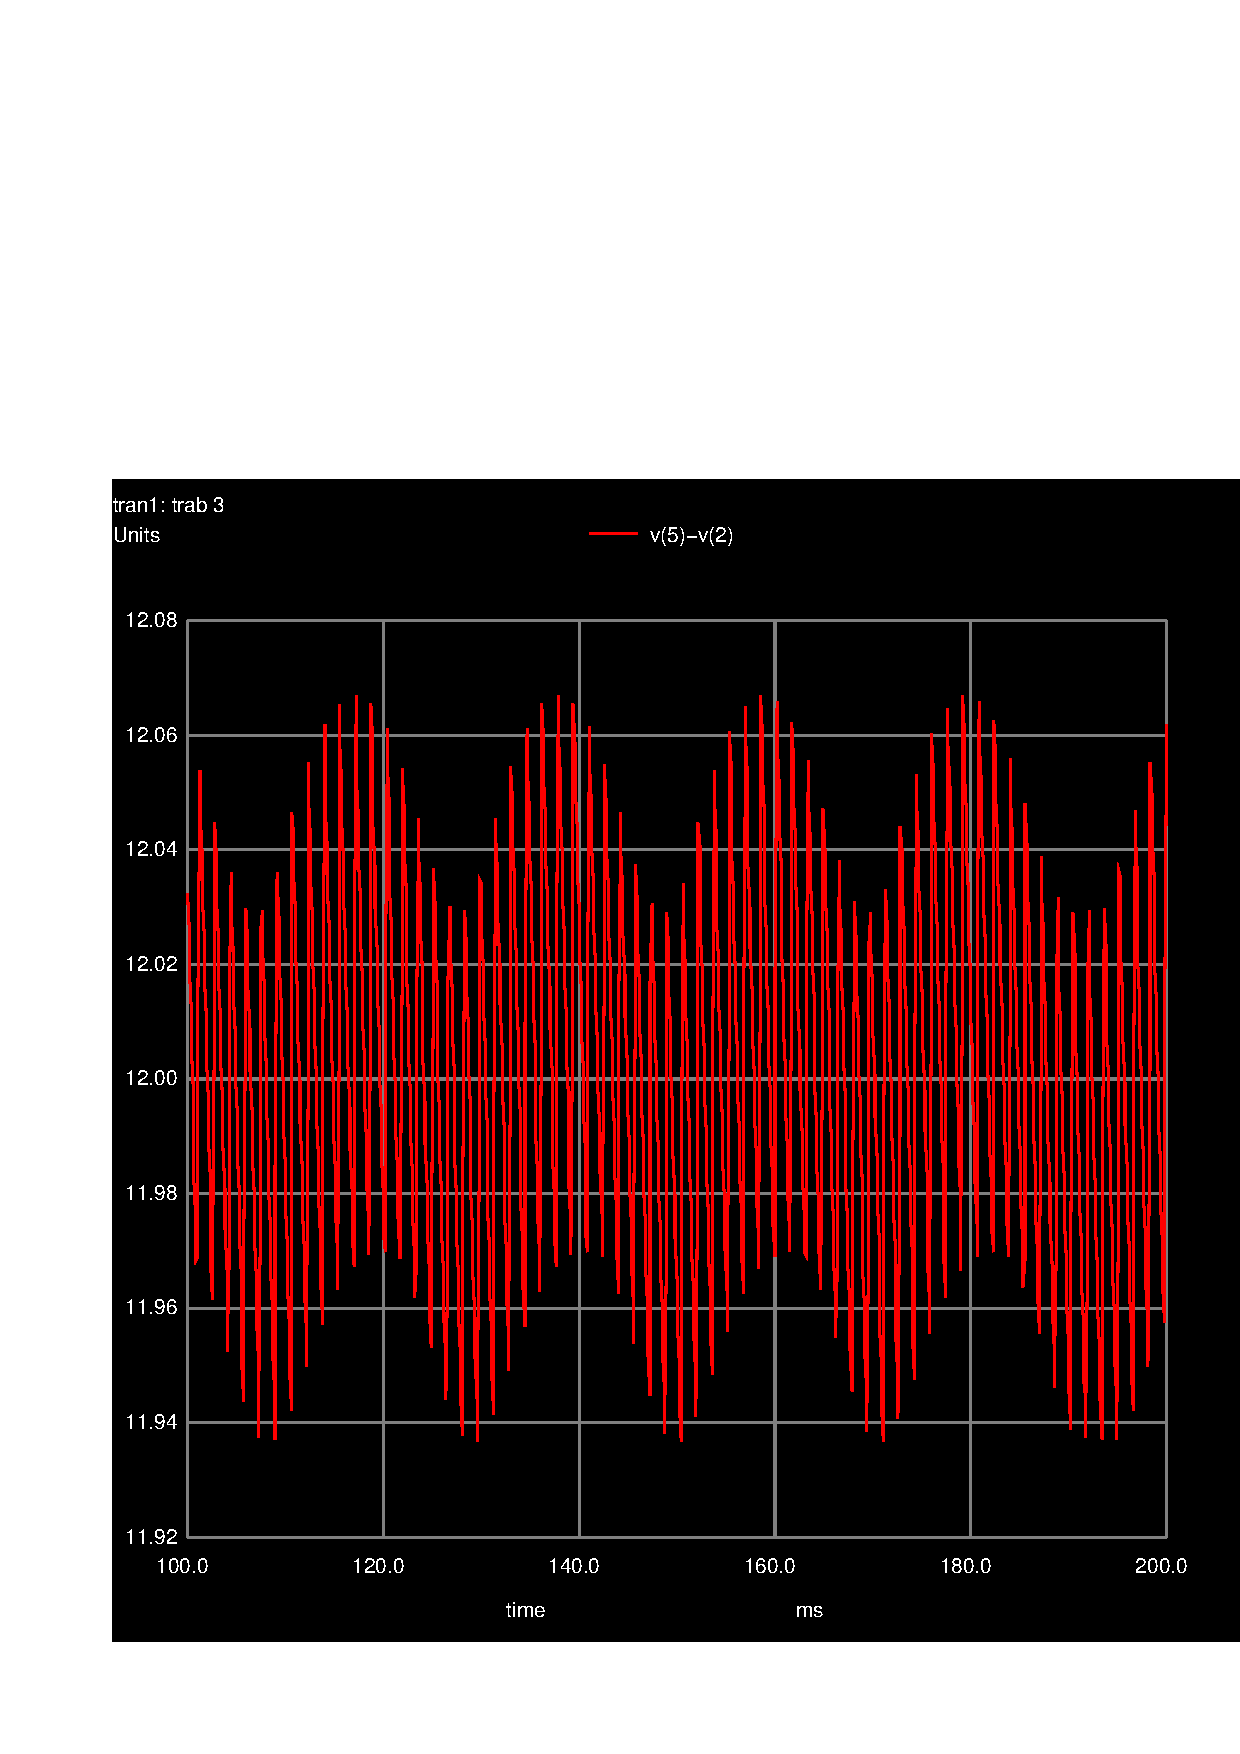
\includegraphics[width = 0.85\linewidth]{sim/zauzau.pdf}
    \vspace*{-10mm}
        \caption{\textit{Plot of the output voltage registered at the output terminals of the voltage regulator circuit}}
    \label{fig:zauzau}
\end{figure}

Comparing the two plots one can conclude that the plots are perfectly similar except on the $y$ axis scale. In fact, the difference between the two plots was caused by the action of our voltage regulator circuit. As the number of diodes was chosen to set an upper limit to the output voltage of the circuit to the desired value $V = 12V$ the difference registered between the two graphs only reflects the effect of that part of the circuit. And in fact, as one can see, the voltage regulator circuit is working as it is supposed to because the voltage that was intially oscillating around $14V$ is oscillating around $12V$ at the output terminals of the voltage regulator.

\subsection{Plotting $v_o - 12$}
Finally, to conclude the simulation analysis (which one can antecipate that allowed to get precise and satisfactory results) and to better understand how the output voltage behaved next to the desired value of $V = 12V$, one plotted the function $V = v_o - 12$:

\vspace{-140px}
\begin{figure}[H]
    \centering
    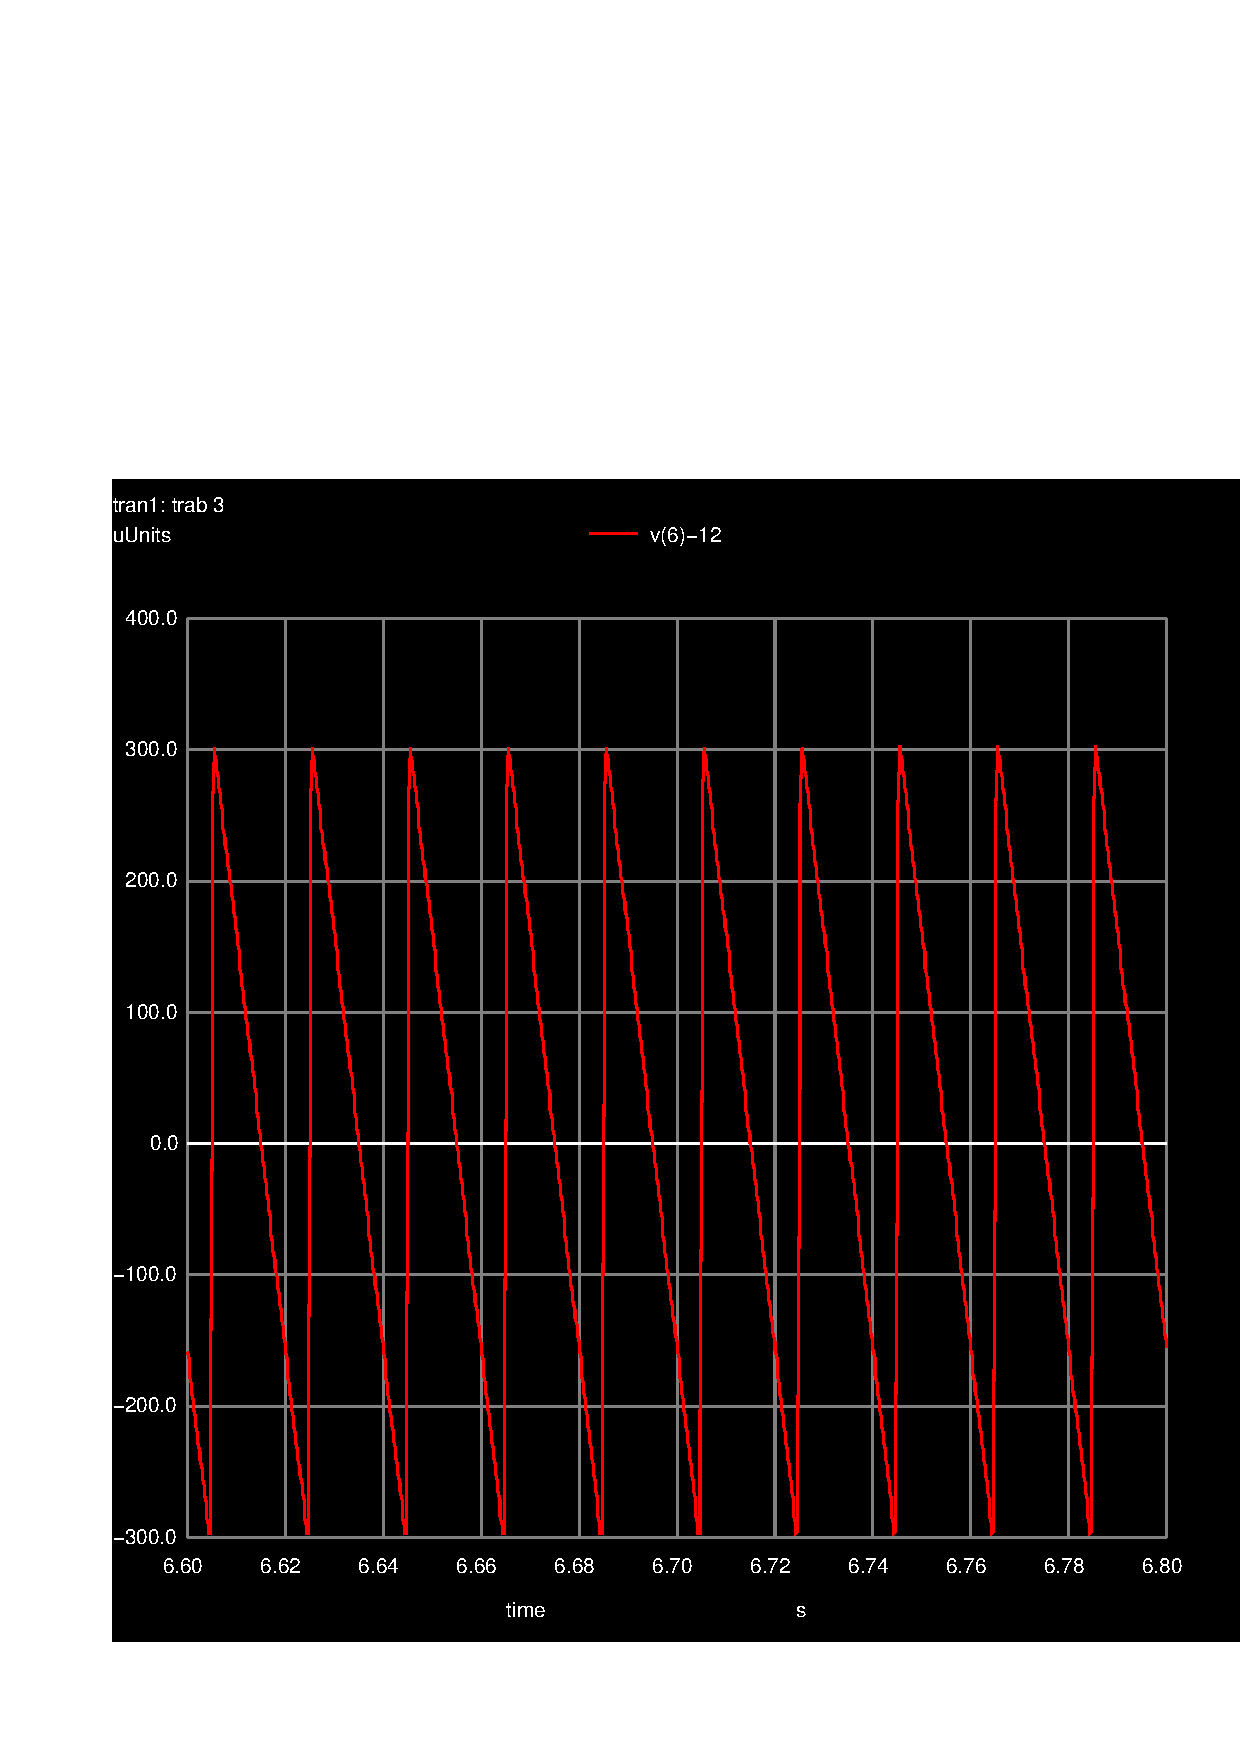
\includegraphics[width = 0.85\linewidth]{sim/deviation.pdf}
    \vspace*{-10mm}
        \caption{\textit{Plot of the difference between the circuit's output voltage and the desired voltage, $V=12V$}}
    \label{fig:dev}
\end{figure}

Summing up, all the numerical values,

\begin{table}[H]
    \centering
    \small
    \begin{tabular}{|c|c|}
          \hline
          Variable & $Value$\\
          \hline
          @cb[i] & 0.000000e+00\\ \hline
@ce[i] & 0.000000e+00\\ \hline
@q1[ib] & 7.022567e-05\\ \hline
@q1[ic] & 1.404513e-02\\ \hline
@q1[ie] & -1.41154e-02\\ \hline
@q1[is] & 5.765392e-12\\ \hline
@rc[i] & 1.411536e-02\\ \hline
@re[i] & 1.411536e-02\\ \hline
@rf[i] & 7.022567e-05\\ \hline
@rs[i] & 0.000000e+00\\ \hline
v(1) & 0.000000e+00\\ \hline
v(2) & 0.000000e+00\\ \hline
base & 2.254108e+00\\ \hline
coll & 5.765392e+00\\ \hline
emit & 1.411536e+00\\ \hline
vcc & 1.000000e+01\\ \hline

          \hline
    \end{tabular}
    \caption{All the values resulting from simulation.}
    \label{tab:all}
    \end{table}

